\documentclass{article}
\usepackage[T1]{fontenc}
\usepackage{lmodern}
\usepackage{graphicx}
\usepackage{amsmath,amssymb}
\usepackage[a4paper,margin=2cm]{geometry}
\usepackage[absolute,overlay]{textpos}
\setlength{\TPHorizModule}{1mm}
\setlength{\TPVertModule}{1mm}
\usepackage[indonesian]{babel}
\usepackage{hyperref}
\setlength{\emergencystretch}{2em}
% unit: Halaman 5

\begin{document}

% === Halaman 5 (llm) ===

\begin{center}
\Huge Hybrid Cryptography
\end{center}

\vspace{80mm}

Sumber: \url{https://www.mayurpahwa.com/2018/12/hybrid-cryptography.html}

\vspace{5mm}

\begin{center}
Rinaldi M/I14020 Kriptografi
\end{center}

% deskripsi: Diagram alur kriptografi hibrida yang menunjukkan proses pengiriman pesan dari Alice ke Bob, melibatkan enkripsi dengan kunci rahasia K, enkripsi kunci K dengan kunci publik Bob (PK_Bob), dan dekripsi kembali menggunakan kunci privat Bob (SK_Bob).
% bbox normalisasi: [0.1700, 0.1800, 0.8800, 0.7500]
\begin{textblock*}{149.10mm}(35.70mm,53.46mm)
\noindent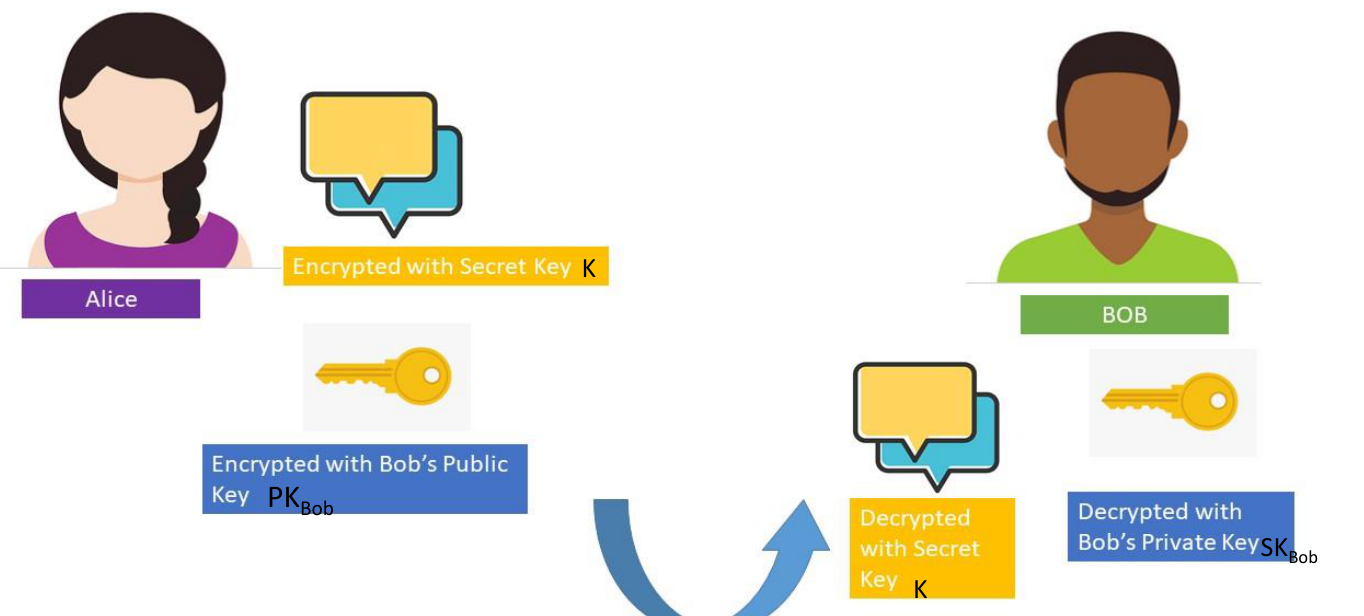
\includegraphics[width=149.10mm,height=169.29mm]{../../images/llm/page_005_img_01.png}%
\end{textblock*}

\end{document}
